%!TEX root = ../INTO-CPS-Manifesto.tex
\section{Background on the Individual Tools}
\label{appendix:tools}
This appendix provides background information on each of the independent tools of the INTO-CPS tool chain.
%
%
%
\subsection{Modelio}\label{app:modelio}
Modelio is a comprehensive MDE \cite{Favre05} workbench tool which supports the UML2.x standard.
%
Modelio adds modern Eclipse-based graphical environment to the solid modelling and generation know-how obtained with the earlier Softeam MDE workbench, Objecteering, which has been on the market since 1991.
%
Modelio provides a central repository for the local model, which allows various languages (UML profiles) to be combined in the same model, abstraction layers to be managed and traceability between different model elements to be established.
%
Modelio makes use of extension modules, enabling the customisation of this MDE environment for different purposes and stakeholders.
%
The XMI module allows models to be exchanged between different UML modelling tools.
%
Modelio supports the most popular XMI UML2 flavors, namely EMF UML2 and OMG UML 2.3.
%
Modelio is one of the leaders in the OMG Model Interchange Working Group (MIWG), due to continuous work on XMI exchange improvements.

Among the extension modules, some are dedicated to IT system architects.
%
For system engineering, SysML or MARTE modules can be used.
%
They provide dedicated modelling support for dealing with general, software and hardware aspects of embedded or cyber physical systems.
%
In addition, several utility modules are available, such as the Document Publisher which provides comprehensive support for the generation of different types of document.

Modelio is highly extendable and can be used as a platform for building new MDE features.
%
The tool enables users to build UML2 Profiles, and to combine them with a rich graphical interface for dedicated diagrams, model element property editors and action command controls.
%
Users can use several extension mechanisms: light Python scripts or a rich Java API, both of which provide access to Modelio‘s  model repository and graphical interface.
%
%
%
\subsection{Overture}\label{app:overture}
The Overture platform \cite{Larsen&10a} is an Eclipse-based integrated development environment (IDE) for the development and validation of system specifications in three dialects of the specification language of the Vienna Development Method.
%
Overture is distributed with a suite of examples and step-by-step tutorials which demonstrate the features of the three dialects.
%
A user manual for the platform itself is also provided \cite{Larsen&13a}, which is accessible through Overture's help system.
%
Although certain features of Overture are relevant only to the development of software systems, VDM itself can be used for the specification and validation of any system with distinct states, known as \emph{discrete-event systems}, such as physical plants, protocols, controllers (both mechanical and software) \emph{etc}.\@, and Overture can be used to aid in validation activities in each case.

Overture supports the following activities:
%
%
%
\begin{itemize}
%
\item  The definition and elaboration of syntactically correct specifications in any of the three dialects, via automatic syntax and type validation.
%
\item  The inspection and assay of automatically generated proof obligations which ensure correctness in those aspects of specification validation which can not be automated.
%
\item  Direct interaction with a specification via an execution engine which can be used on those elements of the specification written in an executable subset of the language.
%
\item  Automated testing of specifications via a custom test suite definition language and execution engine.
%
\item  Visualization of test coverage information gathered from automated testing.
%
\item  Visualization of timing behaviours for specifications incorporating timing information.
%
\item  Translation to/from UML system representations.
%
\item  For specifications written in the special executable subset of the language, obtaining Java implementations of the specified system automatically.
%
\end{itemize}
%
%
%

For more information and tutorials, please refer to the documentation distributed with Overture.

The following is a brief introduction to the features of the three dialects of the VDM specification language.
%
\paragraph{VDM-SL}
This is the foundation of the other two dialects.
%
It supports the development of monolithic state-based specifications with state transition operations.
%
Central to a VDM-SL specification is a definition of the state of the system under development.
%
The meaning of the system and how it operates is conveyed by means of changes to the state.
%
The nature of the changes is captured by state-modifying operations.
%
These may make use of auxiliary functions which do not modify state.
%
The language has the usual provisions for arithmetic, new dependent types, invariants, pre-\@ and post-conditions \emph{etc}.
%
Examples can be found in the VDM-SL tutorials distributed with Overture.
%
\paragraph{VDM++}
The VDM++ dialect supports a specification style inspired by object-oriented programming.
%
In this specification paradigm, a system is understood as being composed of entities which encapsulate both state and behaviour, and which interact with each other.
%
Entities are defined via templates known as \emph{classes}.
%
A complete system is defined by specifying \emph{instances} of the various classes.
%
The instances are independent of each other, and they may or may not interact with other instances.
%
As in object-oriented programming, the ability of one component to act directly on any other is specified in the corresponding class as a state element.
%
Interaction is naturally carried out via precisely defined interfaces.
%
Usually a single class is defined which represents the entire system, and it has one instance, but this is only a convention.
%
This class may have additional state elements of its own.
%
Whereas a system in VDM-SL has a central state which is modified throughout the lifetime of the system, the state of a VDM++ system is distributed among all of its components.
%
Examples can be found in the VDM++ tutorials distributed with Overture.
%
\paragraph{VDM-RT}
VDM-RT is a small extension to VDM++ which adds two primary features:
%
%
%
\begin{itemize}
%
\item  The ability to define how the specified system is envisioned to be allocated on a distributed execution platform, together with the communication topology.
%
\item  The ability to specify the timing behaviours of individual components, as well as whether certain behaviours are meant to be cyclical.
%
\end{itemize}
%
Finer details can be specified, such as execution synchronisation and mutual exclusion on shared resources.
%
A VDM-RT specification has the same structure as a VDM++ specification, only the conventional system class of VDM++ is mandatory in VDM-RT.
%
Examples can be found in the VDM-RT tutorials distributed with Overture.
%
%
%
\subsection{20-sim}\label{app:20sim}
{20-sim} \cite{20sim,Broenink97} is a commercial modelling and simulation software package for mechatronic systems.
%
With {20-sim}, models can be created graphically, similar to drawing an engineering scheme.
%
With these models, the behaviour of dynamic systems can be analysed and control systems can be designed.
%
{20-sim} models can be exported as C-code to be run on hardware for rapid prototyping and HiL-simulation.
%
{20-sim} includes tools that allow an engineer to create models quickly and intuitively.
%
Models can be created using equations, block diagrams, physical components and bond graphs \cite{Karnopp&68}.
%
Various tools give support during the model building and simulation.
%
Other toolboxes help to analyse models, build control systems and improve system performance.
%
%
%
\begin{figure}[hpt!]
	\centerline{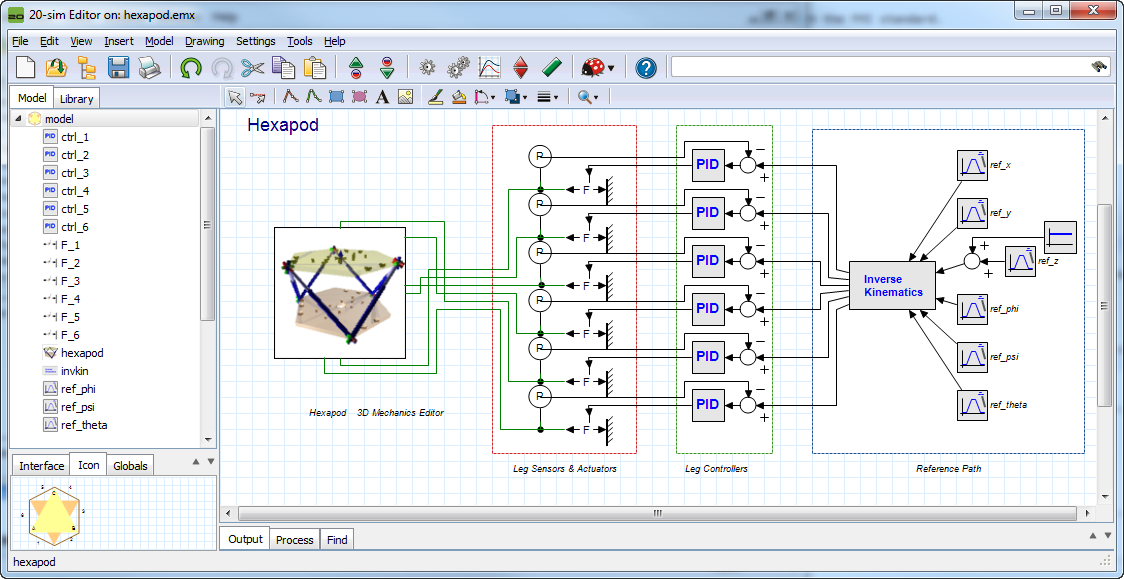
\includegraphics[width=\textwidth]{figures/20-sim_hexapod_model.png}}
	\caption{Example of a hexapod model in 20-sim.}
	\label{figure:20sim_hexapod_example}
\end{figure}
%
%
%
Figure \ref{figure:20sim_hexapod_example} shows {20-sim} with a model of a controlled hexapod.
%
The mechanism is generated with the 3D Mechanics Toolbox and connected with standard actuator and sensor models from the mechanics library.
%
The hexapod is controlled by PID controllers which are tuned in the frequency domain.
%
Everything that is required to build and simulate this model and generate the controller code for the real system is included inside the package.

The {20-sim} Getting Started manual \cite{20simGettingStarted16} contains examples and step-by-step tutorials that demonstrate the features of {20-sim}.
%
More information on {20-sim} can be found at \url{http://www.20sim.com} and in the user manual at \url{http://www.20sim.com/webhelp} \cite{20simReference16a}.
%
The integration of {20-sim} into the INTO-CPS tool-chain is realised via the FMI standard.
%
%
%
\subsection{OpenModelica}\label{app:OM}
OpenModelica \cite{Fritzson04} is an open-source Modelica-based modelling and simulation environment.
%
Modelica \cite{Fritzson&98} is an object-oriented, equation based language to conveniently model complex physical systems containing, e.g., mechanical, electrical, electronic, hydraulic, thermal, control, electric power or process-oriented subcomponents. The Modelica language (and OpenModelica) supports continuous, discrete and hybrid time simulations.
%
OpenModelica already compiles Modelica models into  FMU, C or C++ code for simulation.
%
Several integration solvers, both fixed and variable step size, are available in OpenModelica: euler, rungekutta, dassl (default), radau5, radau3, radau1.

OpenModelica can be interfaced to other tools in several ways as described in the OpenModelica user's manual \cite{OpenModelicaUG15}:
%
%
%
\begin{itemize}
%
\item via command line invocation of the omc compiler
%
\item via C API calls to the omc compiler dynamic library
%
\item via the CORBA interface
%
\item via OMPython interface \cite{Ganeson&12}
%
\end{itemize}
%
%
%
OpenModelica has its own scripting language, Modelica script (mos files), which can be used to perform actions via the compiler API, such as loading, compilation, simulation of models or plotting of results.
%
OpenModelica supports Windows, Linux and Mac Os X.

The integration of OpenModelica into the INTO-CPS tool chain is realised via compliance with the FMI standard, and is described in Deliverable D4.3b \cite{INTOCPSD4.3b}.
%
%
%
\subsection{RT-Tester}\label{app:RTT}
The RT-Tester \cite{VSI-rtt-man} is a test automation tool for automatic
test generation, test 
execution and real-time test evaluation. Key features include a strong
C/C++-based test script language, high performance multi-threading, and
hard real-time capability.
The tool has been successfully applied in avionics, rail automation, and
automotive test projects.
%
In the INTO-CPS tool chain, RT-Tester is responsible for model-based testing, as well as for model checking.
%
This section gives some background information on the tool from these two perspectives.
%
%
%
\subsubsection{Model-based Testing}
% RT-Tester Model Based Extension (RTT-MBT)
The RT-Tester Model Based Test Case and Test Data Generator (RTT-MBT) \cite{VSI-mbt-man} 
supports model-based testing (MBT), that is, automated generation of test cases, test
data, and test procedures from UML\allowbreak{}/SysML models. A number of common modelling
tools can be used as front-ends for this. 
%
The most important technical challenge in model-based test automation is the extraction of test cases from test models.
%
RTT-MBT combines an SMT solver with a technique akin to bounded model checking so as to extract finite paths through the test model according to some predefined criterion.
%
This criterion can, for instance, be MC/DC coverage, or it can be requirements coverage (if the requirements are specified as temporal logic formulae within the model).
%
A further aspect is that the environment can be modelled within the test model.
%
For example, the test model may contain a constraint such that a certain input to the system-under-test remains in a predefined range.
%
This aspect becomes important once test automation is lifted from single test models to multi-model cyber-physical systems.
%
The derived test procedures use the RT-Tester Core as a back-end, allowing the
system under test to be provided on real hardware, software only, or even
just simulation to aid test model development.

Further, RTT-MBT includes requirement tracing from test models down to test executions
and allows for powerful status reporting in large scale testing projects.
%
%
%
\subsubsection{Model Checking of Timed State Charts}
\label{appendix:rtt-model-checking}
RTT-MBT applies model checking to behavioural models that are specified as timed state charts in UML and SysML, respectively.
%
From these models, a transition relation is extracted and represented as an SMT formula in bit-vector theory~\cite{Kroening&08}, which is then checked against LTL formulae~\cite{Pnueli77} using the algorithm of Biere \emph{et al.\@}~\cite{Biere&06}.
%
The standard setting of RTT-MBT is to apply model checking to a single test model, which consists of the system specification and an environment.
%
%
%
\begin{itemize}
%
\item A component called \emph{TestModel} that is annotated with stereotype \emph{TE}.
%
\item A component called \emph{SystemUnderTest} that is annotated with stereotype \emph{SUT}.
%
\end{itemize}
%
%
%
RTT-MBT uses the stereotypes to infer the role of each component.
%
The interaction between these two parts is implemented via input and output interfaces that specify the accessibility of variables using UML stereotypes.
%
%
%
\begin{itemize}
%
\item A variable that is annotated with stereotype \emph{SUT2TE} is written by the system model and readable by the environment.
%
\item A variable that is annotated with stereotype \emph{TE2SUT} is written by the environment and read by the system model as an input.
%
\end{itemize}
%
%
%
A simple example is depicted in \autoref{figure:vsi-simple}, which shows a simple composite structure diagram in Modelio for a turn indication system.
%
The purpose of the system is to control the lamps of a turn indication system in a car.
%
Further details are given in~\cite{rttmbtmanual}.
%
The test model consists of the two aforementioned components and two interfaces:
%
%
%
\begin{itemize}
%
\item {\bf Interface1} is annotated with stereotype \emph{TE2SUT} and contains three variables {\tt voltage}, {\tt TurnIndLvr} and {\tt EmerSwitch}. These variables are controlled by the environment and fed to the system under test as inputs.
%
\item {\bf Interface2} is annotated with stereotype \emph{SUT2TE} and contains two variables {\tt LampsLeft} and {\tt LampsRight}. These variables are controlled by the system under test and can be read by the environment.
%
\end{itemize}
%
%
%
Observe that the two variables {\tt LampsLeft} and {\tt LampsRight} have type {\tt int}, but should only hold values {\tt 0} or {\tt 1} to indicate states \emph{on} or \emph{off}.
%
A straightforward system property that could be verified would thus be that {\tt LampsLeft} and {\tt LampsRight} indeed are only assigned {\tt 0} or {\tt 1}, which could be expressed by the following LTL specification:
%
%
%
\[
\mathbf{G} (0 \leq {\tt LampsLeft} \leq 1 \wedge 0 \leq {\tt LampsRight} \leq 1)
\]
%
%
%
A thorough introduction with more details is given in the RTT-MBT user manual~\cite{rttmbtmanual}.
%
%
%
\begin{figure}
\centerline{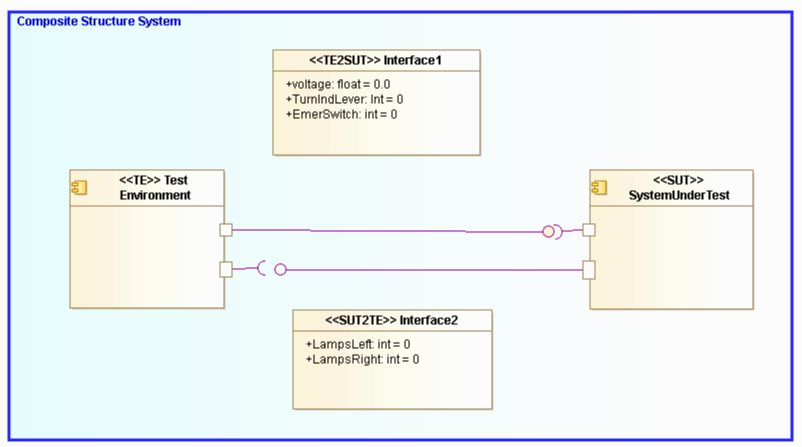
\includegraphics[width=\textwidth]{figures/VSI-modelio_turn_indication_small_toplevel_composite.png}}
\caption{Simple model that highlights interfaces between the environment and
  the system-under-test.}
\label{figure:vsi-simple}
\end{figure}
%
\subsection{4DIAC}\label{app:4DIAC}
%
4diac provides an open source infrastructure for distributed industrial process measurement and control systems based on the IEC 61499 standard. IEC 61499 defines a domain-specific
modeling language for developing distributed industrial control solutions. IEC 61499 extends IEC 61131-1 by improving the encapsulation of software components for increased re-usability, 
providing a vendor-independent format, and simplifying support for controller-to-controller communication. Its distribution functionality and the inherent support for dynamic reconfiguration 
provide the required infrastructure for Industrie 4.0 and industrial IoT applications.
%
The 4DIAC framework allows the development of distributed control systems compliant to the IEC 61499 standard and three of its main projects are:
%
\begin{itemize}
  \item 4DIAC-RTE (FORTE): The runtime environment is a small portable C++ implementation of an IEC 61499 runtime environment, which supports the execution of distributed control programs 
  on small embedded devices. FORTE runs above a device's OS. It is a multi-threaded and low memory consuming runtime environment. The runtime environment has been tested on the following systems:
  \begin{itemize}
    \item Windows Cygwin on i386, ppc and xScale
    \item Linux on i386, ppc and xScale
    \item NetOS
    \item RTOS on IPC@chip
    \item eCos ARM7
    \item VxWorks
    \item freeRTOS
  \end{itemize}     
  \item 4DIAC-IDE: This is the IDE (Integrated Development Environment) written in Java and based on the Eclipse framework and provides an extensible engineering environment for modeling 
  distributed control applications compliant to the IEC 61499 standard. The user uses 4DIAC to create FBs, applications, configure the devices and all related to IEC 61499 and also download this 
  to devices running FORTE.
  \item Function Block Library: contains Function Blocks which are available on the 4DIAC-RTE and can, therefore, be used to create IEC 61499 compliant control applications.
\end{itemize}
%
\begin{figure}[hpt!]
  \centerline{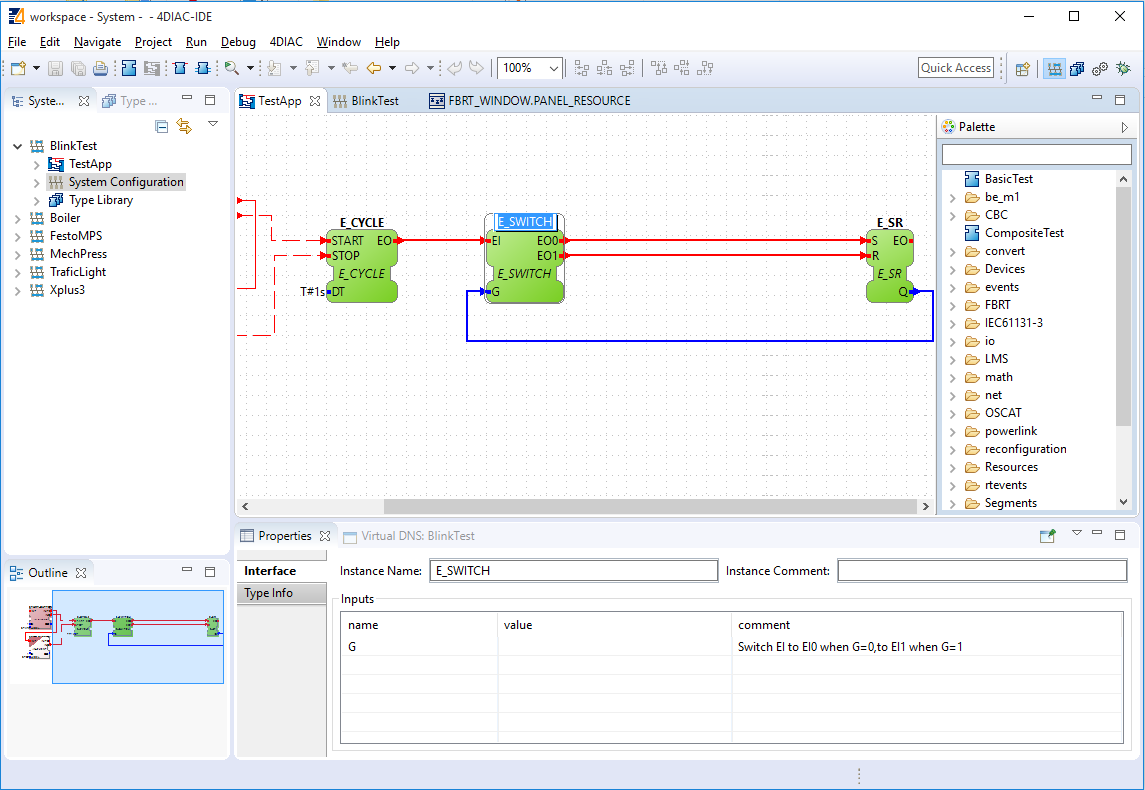
\includegraphics[width=\textwidth]{figures/4diac-overview.png}}
  \caption{Overview of the 4DIAC-IDE}
  \label{figure:4diac-overview}
\end{figure}
%
%
From version 1.10, 4DIAC has the capability to export each device of a system as an FMU (FMI 2.0) in order to test the behaviour of the controller against another FMU of the controlled system in 
the co-simulation environment. More detailed information about 4DIAC can be found in the official website:
%
\begin{quote}
  \url{http://www.eclipse.org/4diac/en_help.php}
\end{quote} 
%
%
\subsection{AutoFOCUS-3}

\fbox{Hernan Ponce de Leon}
